\documentclass[14pt, a4paper,oneside]{extarticle}
\usepackage[T1,T2A]{fontenc}
\usepackage[utf8]{inputenc}
\usepackage[russian]{babel}
\usepackage{epstopdf}
\usepackage{verbatim}
\usepackage[linesnumbered,boxed]{algorithm2e}
\usepackage[]{graphicx}
\usepackage{setspace}

\usepackage{indentfirst}
\usepackage{hyperref} %url

\usepackage{amsmath} 
 \setcounter{tocdepth}{2} 
\usepackage{floatrow}
% Table float box with bottom caption, box width adjusted to content
\newfloatcommand{capbtabbox}{table}[][\FBwidth]

\onehalfspacing

%\graphicspath{{image/}}
\usepackage[left=2cm,right=2cm,bottom=3cm,top=2cm]{geometry}
\bibliographystyle{unsrt}
\SetKwProg{Op}{Operator}{}{}
\SetKwProg{Func}{Function}{}{}
\SetAlgoNlRelativeSize{0}
\author{Швецов Денис}
\title{Реферат по английскому}
\begin{document}
\thispagestyle{empty}

	\thispagestyle{empty}
	
	\begin{center}
		\ \vspace{-0.5cm}
		
		
\includegraphics[width=0.5\textwidth]{msu}\\
		{Московский государственный университет имени М.В. Ломоносова}\\
		Факультет вычислительной математики и кибернетики\\
		Кафедра автоматизации систем вычислительных комплексов
		
		\vspace{2.5cm}
		
		{\Large ШВЕЦОВ Денис Андреевич}
		
		\vspace{1cm}
		
		{\Large\bfseries
			Алгоритмы управления перегрузками в центрах обработки данных\\}
		
		\vspace{2cm}
		
		{\large РЕФЕРАТ}
	\end{center}
	\vfill
	\begin{center}
		Москва, 2017
	\end{center}
	\vspace{1cm}
	\enlargethispage{4\baselineskip}

\newpage
	\addcontentsline{toc}{section}{Оглавление}
	\tableofcontents
\newpage
\section{Введение}

На сегодняшний день центры обработки данных являются важнейшей частью инфраструктуры организаций предоставляющие всевозможные он-лайн сервисы для своих клиентов, например, веб-поиск, торговые площадки, рекомендательные системы. Качество работы этих сервисов напрямую влияет на количество заинтересованных пользователей и следственно на доход. 

Приложения он-лайн сервисов должны работать в реальном времени~--- пользователь вводит запрос в веб-браузере и ожидает незамедлительного отклика (время отклика не должно превышать 300 миллисекунд). 
Так же приложения работают с большими объемами данных (например, весь веб-индекс) для формирования ответа на запрос. Обычно эти данных распределены между тысячами сервером и каждый запрос попадает на все сервера.

Высокие нагрузки на центры обработки данных и жесткие требования приложений порождают жесткие требования на сети в центрах обработки данных. Работа приложений в реальном времени требует низких задержек в сети и устойчивости к разрывам. Также поскольку приложениям надо постоянно обновлять внутренние структуры данных сети должны иметь высокую пропускную способность для длительных потоков. При этом, несмотря на предъявленные требования, в сетях центров обработки данных зачастую используется дешевое сетевое оборудование, например, ToR (Top of the rack) коммутатор, который соединяет между собой сервера в стойке, имеет 48 портом скоростью 1 гигабит в секунду.

В условиях сетей центров обработки данных TCP протокол не достаточно хорошо справляется с поставленными требованиями~\cite{dctcp}, поэтому ведутся работы по разработке протоколов управления перегрузками в центрах обработки данных.
Cуществуют подходы, в которых используются возможности протокола TCP, такие как ECN метка~\cite{dctp, d2tcp}, при этом остальные функции протокола остаются нетронутыми.
Параллельно с этим существуют работы, в которых, разрабатывают протоколы не совместимые с TCP~\cite{d3tcp}, например, Facebook разработала свой протокол управления перегрузками поверх UDP~\cite{facebook}.

\newpage

\section{Центры обработки данных}
\subsection{Приложения центров обработки данных}

На сегодняшний день крупномасштабные приложения в центрах обработки данных используют разработаны в соответствии с подходом разделение/агрегация (см. рисунок % partition/aggreagate pattern
Запрос с уровней, расположенных наверху, делится на части и передаются на нижний уровень обрабатывающем процессам. Ответ от этих обрабатывающих процессов агрегируется для получения результирующего ответа. Такой подход используется даже в таких сервисах обработки данных как MapReduce и  Dryad. % Может быть и тут ссылки вставаить

Интерактивная природа веб-приложений означает, что задержка это значимый параметр. Приложения обычно имеют ограничения в 200-300 миллисекунд для того, чтобы завершить свои вычисления и вернуть ответ пользователю~\cite{sla}. Это ограничение ведет к тому приводят к ограничениям на задержку на каждом уровне иерархии центров обработки данных. Эти ограничения означают, что сетевые потоки, которые несут в себе запросы и ответы к узлам и от них, имеет директивные интервалы выполнения, и если какой-то узел не уложился в свой директивный интервал, вычисления продолжаются без его ответа, что снижает качество результата, не говоря уже о бесполезном использовании пропускной способности сети.

\subsection{Сетевая нагрузка в центрах обработки данных}
Были проведены исследования о том, какой трафик существует в центрах обработки данных~\cite{dctcp}, были выделены три различных типов трафика:
\begin{enumerate}
\item трафик запросов
\item трафик коротких сообщений, который координирует активность в центре обработки данных
\item фоновый трафик, который передает большие объемы данных между серверами для того, чтобы приложения поддерживали внутренние структуры в актуальном состоянии и выдали ответы высокого качества.
\end{enumerate}

\paragraph{Трафик запросов.}
Трафик запросов использует модель разделения агрегации и состоит из очень коротких потоков, критичных к задержке. Агретор высшего уровня разделяет запрос на большое количество агрегаторов среднего уровня, которые в свою очередь деляет каждый запрос на 43 других сервера, находящийся в той же самой стойке. Размеры трафика запросов достаточно постоянный~--- 1,6 килобайт для запросов и 1,6-2 килбоайта для ответов.
% Можно еще припихнуть картинку про распределение времени между двумя запросами

\paragraph{Фоновый трафик.}
\begin{figure}
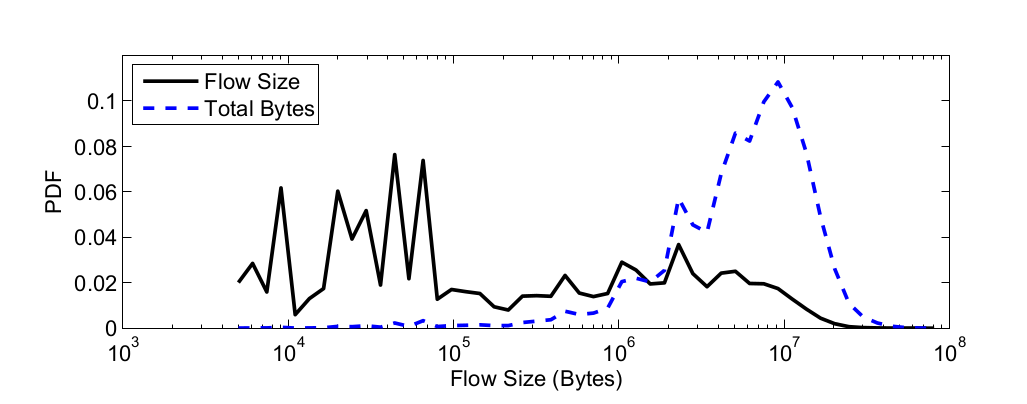
\includegraphics[width=\linewidth]{pdf_of_flow_size.png}
\caption{Плотность вероятности размера потока для фонового трафика. Плотность вероятности общего количество данных показывает вероятность того, что случайно выбранный байт будет принадлежать потоку данного размера.}
\label{pdf_of_flow_size}
\end{figure}

Параллельно с трафиком запросов существует фоновый трафик, состоящий и из больших и из маленьких потоков. % Плостность распредления потоков
На рисунке~\ref{pdf_of_flow_size} видно, что большинство фоновых потоков имеет маленький размер, но большинство данных в фоновом трафике принадлежит большим потокам.
%TODO Дописать эту часть

\subsection{Проблемы сетей в центрах обработки данных}

Большинство коммутаторов в центрах обработки данных это \emph{коммутаторы с разделяемой памятью}, использующие статического мультиплексирования с помощью буфера пакетов доступного для всех портов коммутатора. Пакет прибывает на интерфейс и сохраняется в высокоскоростную память разделенную между всеми интерфейсами. Устройство управления памятью динамически выделяет для пакета память. Устройство управления памятью старается дать интерфейсу столько памяти, сколько ему необходимо, динамически настраивая максимальный объем памяти, который может использовать любой интерфейс.
Если пакет должен быть поставлен в очередь на отправку на некоторый интерфейс, но этот интерфейс достиг максимума выделенной ему памяти или истощился сам пул свободной разделяемой памяти, тогда пакет будет отброшен. Создание разделяемой памяти большого объема очень дорогой процесс, поэтому большинство дешевых коммутаторов имеют \emph{маленький буфер пакетов}. Этот маленький буфер пакетов является причиной трех специфичных проблем, которые описаны далее.

\paragraph{Incast}

Incast это модель общения в сетях, в которой от многих отправителей пакет адресован одному получателю. Если на коммутаторе много потоков выходят на одном и том же интерфейсе в один и тот же период времени, пакеты могут израсходовать всю выделенную на интерфейс память, что приведет к потере пакетов. Это может произойти даже если потоки небольшие. Такой трафик естественным образом возникает в центрах обработки данных из-за использование модели разделение/агрегация, запросы поступают на обрабатывающие процессы в одно и то же время, и процессы отвечают примерно в тоже время, что и создает проблему Incast трафика.

При этом так как размер каждого отдельного ответа приложения достаточно мал (в проведенном исследовании~\cite{dctcp} он составляет 2 килобайта, что умещается в два пакета) потеря пакета почти не оказывает влияния на время ожидания переотправления пакета в TCP. Если выставить минимальное время ожидания перепосылки пакета равным одному RTT это будет примерно 300 миллисекунд, следовательно если случается потеря пакета ответ приложения практически всегда не укладывается в свой директивный интервал.

Разработчики сделали два основных изменения а коде приложений, чтобы избежать тайм-аутов для ответов обрабатывающих процессов.
\begin{enumerate}
\item во-первых они явно ограничили размер ответ двумя килобайтами, чтобы улучшить шансы того, что все ответы уместятся в памяти коммутатора,
\item во-вторых разработчики добавили джитеринг~\cite{jittering} в уровень приложений, чтобы десинхронизовать ответы приложений с помощью задержки ответа приложения на некоторое случайное время, или использовали слоттирование времени ответа для тех же целей~\cite{ictcp}.
\end{enumerate}
%То, что уменьшение RTO_min не помогает

\paragraph{Загрузка очереди.}
Длительные и большие TCP потоки могут являться причиной того, что длина очереди в узком месте на коммутаторе будет расти до тех пор, пока пакет не начнут отбрасываться приводя к <<пилообразному>> процессу изменения скорости передачи (см рис.~\ref{tcp_sawtooth}).
\begin{figure}
	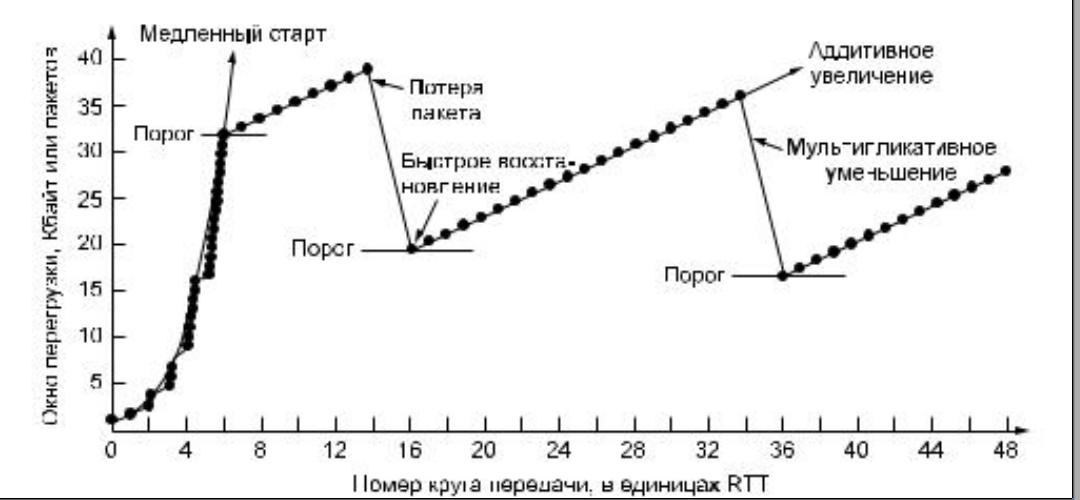
\includegraphics[width=\linewidth]{tcp_sawtooth.jpg}
	\caption{Пилообразный график скорости передачи TCP}
	\label{tcp_sawtooth}
\end{figure}
Учитывая тот факт, что длительные и короткие потоки обрабатываются в одной и той же очереди, можно выделить две проблемы. Во-первых, потеря пакетов в коротких потоках может привести к проблеме Incast трафика. Во-вторых, даже если потери пакетов не было, короткие потоки испытывает б\'{о}льшие задержки, так как они находятся в очереди за пакетами длительных и больших потоков. Так как каждый обрабатывающий процесс в центре обработки данных работает и с трафиком запросов и с фоновым трафиком, такое состояние может случаться довольно часто.

Исследования~\cite{dctcp} показали, что в центрах обработки данных с классическим TCP, короткие потоки в самом деле испытывают неприемлимые задержки из-за длинной очереди на коммутаторе (до 14 миллисекунд). При этом потери пакетов не было, так что единственный способ борьбы с такой задержкой  это уменьшение очереди.

\paragraph{Переполнение буфера.}
В центре обработке данных сосуществует смесь длительных и коротких потоков, и очень частая ситуация, когда короткие потоки на одном порту испытывают влияние активностью на любом из других портов. Коэффициент потерь коротких потоков зависит от числа длительных потоков, проходящих через другие порты. Это происходит из-за того, что активность на разных портах разделяет между собой общую память.

Длительные и жадные TCP потоки заполняют очередь на своих интерфейсах. Так как пространство буфера это разделяемый ресурс, заполнение очереди уменьшает доступное пространство памяти для того избегать разрывов потоков. В результате происходит потеря пакетов, так же как и в проблема Incast трафика, но даже с рассинхронными потоками.
\newpage

\subsection{Директивные интервалы}

TCP не использует тот факт, что у приложений в центрах обработки данных, имеют сроки выполнения, и разделяет пропускную способность равномерно между всеми потоками, игнорируя их директивные интервалы. Использование знания о директивных интервалах потоков может помочь в двух случаях~\cite{d3tcp}:
\begin{enumerate}
\item \emph{случай несправедливого разеления пропускной способности}: 
Предположим, что два потока, разделяют между собой один канал связи, который является узким местом, один из этих потоков имеет более сжатый директивный интервал, чем другой. С
\end{enumerate}


\section{Алгоритмы управления перегрузками}
\subsection{Data Center TCP (DCTCP)}
Основная цель Data Center TCP (DCTCP)~--- достигнуть высокой пропускной способности, устойчивости к разрывам и низкой задержки в центрах обработки данных на коммутаторах с маленьким буфером. Поэтому при DCTCP поддерживает маленькую загрузку очереди на коммутаторе при той же пропускной способности.

DCTCP достигает поставленных целей напрямую реагируя перегрузке пропорционально ее степени. Для этого используется схема маркирования пакетов на коммутаторах меткой \emph{Congestion Experinced (CE)} как только размер занятного буфер превысил некоторый небольшой порог. DCTCP отправитель реагирует на это, уменьшая TCP окно перегрузки на значение зависящее от доли маркированных пакетов: чем больше доля маркрованных пакетов, тем больше значение, на которое уменьшится окно перегрузки.

Важно заметить, что ключевым компонентом в DCTCP является не правила управления перегрузками как таковые, а то, каким образом многобитовая информация представляется в последовательности однобитовых меток пакетов. И так как DCTCP требует от сети только один бит в пакете для передачи своей информации, можно использовать технологию Explicit Congestion Notification (ECN), которая доступна в большинстве современных коммутаторах и TCP стеках.

Алгоритм DCTCP состоит из трех основных компонент:
\begin{enumerate}

\item
во-первых, маркирование пакетов на коммутаторах.
DCTCP использует очень простую схему управления очередью. Есть только один параметр~--- порог маркирования $K$. Прибывший пакет маркируется CE меткой, если размер занятой очереди больше чем $K$, иначе он не маркируется. Это схема обеспечивает быстрое информирование отправителя о том, что очередь переполняется. Можно адаптировать механизм Random Early Detection (RED)~\cite{red} для DCTCP, достаточно просто выставить нижние и верхние пороги равными K;
\item
во вторых, ответ с ECN меткой на получателе. 
Единственное различие между TCP получателем и DCTCP получателем, заключается в том, каким образом информация о CE метках отправляется обратно на отправителя. RFC 3168 устанавливает, что получатель отправляет набор ECN меток в серии подтверждений полученных пакетов до тех пор, пока он не получит отправитель не сообщит, что эти метки были получены.
В то время как DCTCP получатель пытается передать точную последовательность CE меток отправителю. Самый простой способ сделать это, помечать пакет с подтверждением меткой ECN тогда и только тогда, когда полученный пакет помечен CE меткой.

Тем не менее использовать технику отложенного подтверждения получения пакета (одно подтверждение на несколько полученных пакетов) важно по многим причинам, включая уменьшение нагрузки на отправителя. Чтобы поддерживать отложенное подтверждение DCTCP использует детерминированный конечный автомат с двумя состояниями, для того отправки подтверждения (см. рис.~\ref{state_machine}).
\begin{figure}
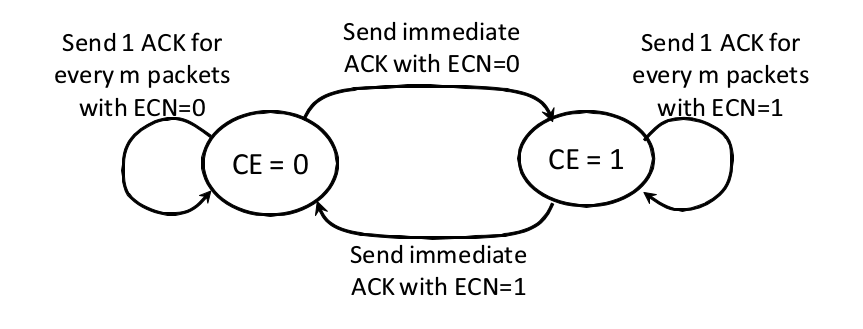
\includegraphics[width=\linewidth]{state_machine.png}
\caption{Конечный автомат отправки подтверждения получения пакета}
\label{state_machine}
\end{figure}
Так как отправитель знает, сколько отправленных полученное подтверждение покрывает, он может точно восстановить сколько маркированных пакетов пришло к получателю.

\item
Контролирование окна перегрузок на отправителе.
Отправитель оценивает долю пакетов, которые были помечены, обозначенную за $\alpha$. Данная переменная обновляется через каждое окно переданных данных (равное примерно одному RTT) следующим образом:
\begin{equation} \label{eq:alpha_update}
\alpha \leftarrow (1 - g) \times \alpha + g \times F,
\end{equation}
где $F$ это доля пакетов, которые были помечена в прошлом окне, и $0 < g < 1$ это вес полученной новой информации по отношению к уже установленному значению $\alpha$. При условии, что отправитель получает маркированные пакеты, только когда длина очереди больше чем $K$ и не получает маркированных пакетов, когда длина очереди меньше, выражение~\eqref{eq:alpha_update} означает, что $\alpha$ оценивает вероятность того, что размер очереди больше чем $K$. Значение $\alpha$ близкое у нулю означает низкий уровень перегрузок, в то время как значение $\alpha$ близкое к единице означает высокий уровень перегрузок.

Единственная разница между отправителем в DCTCP и отправителем в TCP, это то, каким образом они реагируют на получение подтверждения, остальные возможности, такие как как медленный старт, аддитивное увеличение для управления перегрузками, или перепосылка потерянных пакетов остаются такими же.
Но, в то время как TCP всегда уменьшает окно перегрузок в два раза в ответ на полученное маркированное подтверждение, DCTCP использует значение $\alpha$
\begin{equation} \label{eq:cwnd}
cwnd \leftarrow cwnd \times (1 - \alpha/2)
\end{equation}
Таким образом, когда значение $\alpha$ близко к нулю (низкий уровень перегрузок), окно перегрузок уменьшается лишь немного. Другими словами, DCTCP отправитель начинает аккуратно уменьшать окно перегрузок сразу же, как размер очереди превысит $K$. Таким образом DCTCP поддерживает маленькую загрузку очереди, при этом сохраняя высокую пропускную способность. Когда же уровень перегрузок высокий ($\alpha = 1$), DCTCP уменьшает окно перегрузок в два раза, так же как и TCP.
\end{enumerate}

Автора DCTCP анализировали параметры своего алгоритма, они исходили из предположения, что существует $N$ бесконечно длительных потоков с одинаковой круговой задержкой $RTT$, которые делят между собой одно соединение вместимостью $C$? и пришли к следующим выводам:
\begin{enumerate}
\item порог маркирования $K > \frac{C \times RTT}{7}$
\item вес новой информации о о доле помечанных пакетов $g < \frac{1.386}{\sqrt{2(C \times RTT + K)}}$
\end{enumerate}

%Применение DCTCP дает следующие преимущества:
%\begin{enumerate}
%\item
%DCTCP отправитель начинает реагировать на перегрузку сразу же, как только длина очереди на интерфейсе превысит порог $K$, это уменьшает задержки в очереди
%\end{enumerate}

\subsection{Deadline-Driven Delivery control protocol (D\textsuperscript{3})}


\newpage




\begin{thebibliography}{9}
\addcontentsline{toc}{section}{\bibname}

\bibitem {dctcp}
Alizadeh M., Greenberg A., Maltz
 D.A., Padhye J., Patel P., Prabhakar B., 
Sengupta S., and Sridharan M. Data Center TCP (DCTCP) // ACM SIGCOMM 
Computer Communication Review -
 SIGCOMM '10, Volume 40 Issue 4. Oct. 
2010. Pp. 63
-74.

\bibitem {d3tcp}
Wilson C., Ballani H., Karagiannis T., Rowtron
 A. Better never than late: meeting 
deadlines in datacenter networks // ACM SIGCOMM Computer Communication 
Review 
- SIGCOMM '11 Volume 41 Issue 4. Aug. 2011. Pp. 50
-61. 

\bibitem {d2tcp}
Vamanan B., Hasan J., Vijaykumar T.N. Deadline
-aware datacenter tcp (D2TCP) 
// Proceedi
ngs of the ACM SIGCOMM 2012 conference on Applications, 
technologies, architectures, and protocols for computer communication. Aug. 
2012. Pp. 115
-126. 

\bibitem {facebook}
Nishtala R. et al. Scaling Memcache at Facebook //nsdi. – 2013. – Т. 13. – С. 385-398.

\bibitem {sla}
DeCandia G. et al. Dynamo: amazon's highly available key-value store //ACM SIGOPS operating systems review. – 2007. – Т. 41. – №. 6. – С. 205-220.

\bibitem {jittering}
Floyd S., Jacobson V. The synchronization of periodic routing messages //IEEE/ACM transactions on networking. – 1994. – Т. 2. – №. 2. – С. 122-136.

\bibitem {ictcp}
Wu H. et al. ICTCP: Incast congestion control for TCP in data-center networks //IEEE/ACM transactions on networking. – 2013. – Т. 21. – №. 2. – С. 345-358.

\bibitem {red}
Floyd S., Jacobson V. Random early detection gateways for congestion avoidance //IEEE/ACM Transactions on Networking (ToN). – 1993. – Т. 1. – №. 4. – С. 397-413.

\end{thebibliography}

\end{document}